\documentclass{standalone}

\usepackage{tikz}
\usetikzlibrary{matrix,positioning,shapes.arrows,arrows.meta}

\tikzset{ 
table/.style={
  matrix of nodes,
  row sep=-\pgflinewidth,
  column sep=-\pgflinewidth,
  nodes={rectangle,draw,text width=3.25ex,align=center},
  text depth=0.75ex,
  text height=2ex,
  nodes in empty cells
  },
%texto/.style={font=\footnotesize\sffamily},
%title/.style={font=\small\sffamily}
}
\begin{document}
    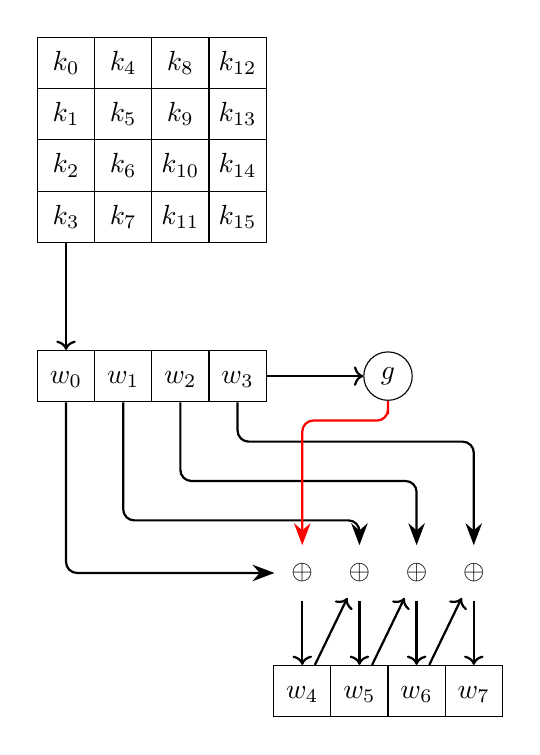
\begin{tikzpicture}[node distance=3cm]
        \matrix [table] (key)
        {
            $k_0$ & $k_4$ & $k_8$ & $k_{12}$ \\
            $k_1$ & $k_5$ & $k_9$ & $k_{13}$ \\
            $k_2$ & $k_6$ & $k_{10}$ & $k_{14}$ \\
            $k_3$ & $k_7$ & $k_{11}$ & $k_{15}$ \\
        };

        \matrix [table, below of=key] (W0)
        {
            $w_0$ & $w_1$ & $w_2$ & $w_3$ \\
        };

        \node [circle, draw, right of=W0] (g) {$g$};

        \matrix [table, below of=g, node distance=4cm] (W1)
        {
            $w_4$ & $w_5$ & $w_6$ & $w_7$ \\
        };

        \node [circle, above of=W1-1-1, node distance=1.5cm] (x1) {$\oplus$};
        \node [circle, above of=W1-1-2, node distance=1.5cm] (x2) {$\oplus$};
        \node [circle, above of=W1-1-3, node distance=1.5cm] (x3) {$\oplus$};
        \node [circle, above of=W1-1-4, node distance=1.5cm] (x4) {$\oplus$};

        \draw[arrows=-{Stealth[scale=1.2]}, rounded corners, thick] (W0-1-1.south) |- ++(0,-1) |- (x1);
        \draw[arrows=-{Stealth[scale=1.2]}, rounded corners, thick] (W0-1-2.south) |- ++(1,-1.5) -| (x2);
        \draw[arrows=-{Stealth[scale=1.2]}, rounded corners, thick] (W0-1-3.south) |- ++(1,-1) -| (x3);
        \draw[arrows=-{Stealth[scale=1.2]}, rounded corners, thick] (W0-1-4.south) |- ++(1,-0.5) -| (x4);
        \draw[arrows=-{Stealth[scale=1.2]}, rounded corners, thick, color=red] (g.south) |- ++(0,-0.25) -| (x1);

        \draw[->, thick] (key-4-1.south) -- (W0-1-1.north);
        \draw[->, thick] (W0-1-4) -- (g);
        \draw[->, thick] (x1) -- (W1-1-1);
        \draw[->, thick] (x2) -- (W1-1-2);
        \draw[->, thick] (x3) -- (W1-1-3);
        \draw[->, thick] (x4) -- (W1-1-4);

        \draw[->, thick] (W1-1-1) -- (x2);
        \draw[->, thick] (W1-1-2) -- (x3);
        \draw[->, thick] (W1-1-3) -- (x4);
    \end{tikzpicture}
\end{document}